\documentclass[10pt, letterpaper]{article}
\usepackage{graphicx}

\usepackage[bottom=1.0in]{geometry}
\topmargin=-0.9in
\oddsidemargin -.3in
\evensidemargin -0.3in
\textwidth=7.0in
%\itemsep= -0.5in
%\parsep= -0.04in

\usepackage[cmex10]{amsmath}
\author{Madhusudan Govindraju}
\date{}
\begin{document}
\title{Biometric Identification - Project2}
\maketitle

\section{K-Nearest Neighbors Classifier } 

\vspace{10mm}

\subsection{Euclidean distance}

The function {\sl find}\_{\sl eucledian()} is written to measure the euclidean distance between two images. All the euclidean distances are stored in an array. For each image in the test data, the the least {\sl K} euclidean distances are sorted out and their counts are taken are weights. Thus the one with the maximum count has the highest vote for the test data and its's label is assigned to the test data. The error rates for the various {\sl training data:test data} ratios are given in Table 1. The graph for K vs error rate has been given in 
fig \ref{fig:3isto1Ratio_varyingK} ( ratio used is 3:1). \\{\sl Weight used} : The class with the maximum count among the K nearest has the highest weight.
   
 
 Steps To run the code :
\begin{verbatim}
>> [imgs_test labels_test] = readMNIST('t10k-images.idx3-ubyte','t10k-labels.idx1-ubyte',1000, 1);
>> [imgs_training labels_training] = readMNIST('train-images.idx3-ubyte','train-labels.idx1-ubyte',
						3000, 52);
>> [class eucl_Dist] = FindClass(imgs_test,imgs_training,3, labels_training, 1000, 3000);
>> [errorRate errors] = finderror(class, labels_test, 1000);
\end{verbatim}
   
   \vspace{10mm}
   

\subsection{Hamming Distance}
Hamming distance is percentage how much the pixels in the image differ. The image is first rearranged to a 2D array of size samplesizex400 with the function{\sl [img] = rearrange(img)}. The hamming distance is calculated between each pixels of the test image and the training image. The labels corresponding to the least K distances obtained from the above step are the nearest neighbors. Those labels are taken and the one with the highest count is assigned to the test image. In case there is a tie. The first label among the ones tied is always chosen.  The fig \ref{fig:varyingK} gives the relation between the error and the size of K.
\\{\sl Weight used} : The class with the maximum count among the K nearest has the highest weight.

Steps To Run the code:
\begin{verbatim}
>> [imgs_training labels_training] = readMNIST('train-images.idx3-ubyte','train-labels.idx1-ubyte',
				3000, 30);
>> [imgs_test labels_test] = readMNIST('t10k-images.idx3-ubyte','t10k-labels.idx1-ubyte',1000, 30);
>> [imgs_test] = rearrange(imgs_test);
>> [imgs_training] = rearrange(imgs_training);
>> [class eucl_Dist] = FindClass_hamming(imgs_test,imgs_training,2, labels_training, 1000, 3000);
>> [eR_3isto1_hamm errors] = finderror(class, labels_test, 1000);
\end{verbatim}



\subsection{City Block Distance}
The City Block distance between two points is the sum of the absolute differences of their Cartesian coordinates. This is also referred to as the taxicab geometry. The image is first rearranged to a 2D array of size samplesizex400 using the function {\sl [img] = rearrange(img)} . The city block distance is calculated between each pixels of the test image and the training image. The labels corresponding to the least K distances obtained from training images are  the nearest neighbors. Their labels are taken and the one with the highest count is assigned to the test image.  The fig \ref{fig:cb_varyingK} gives the relation between size of K and error rate. The ratio used is 3 is to 1.
\\{\sl Weight used} : The class with the maximum count among the K nearest has the highest weight.

Steps To Run the code:
\begin{verbatim}
[ errorRate, class , city_Dist ] = FindClass_City(3,1000 , 3000);
\end{verbatim}
Here the first argument is the value for "K". The second argument is the test data size and the third argument is the training data size.


 \begin{figure}
    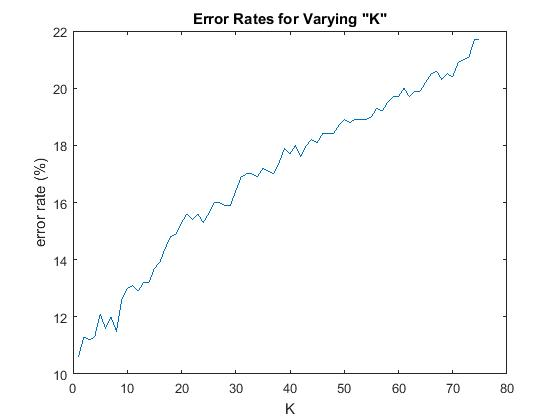
\includegraphics[width=\linewidth]{images/3isto1Ratio_varyingK}
    \caption{ K vs ErrorRate - Euclidean distance}
    \label{fig:3isto1Ratio_varyingK}
    \end{figure}
    
    \begin{figure}
    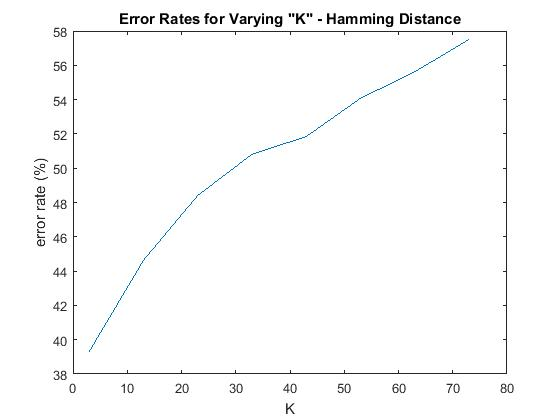
\includegraphics[width=\linewidth]{images/hamm_varyingK}
    \caption{ K vs ErrorRate - Hamming Distance distance}
    \label{fig:varyingK}
    \end{figure}
    
\begin{figure}
    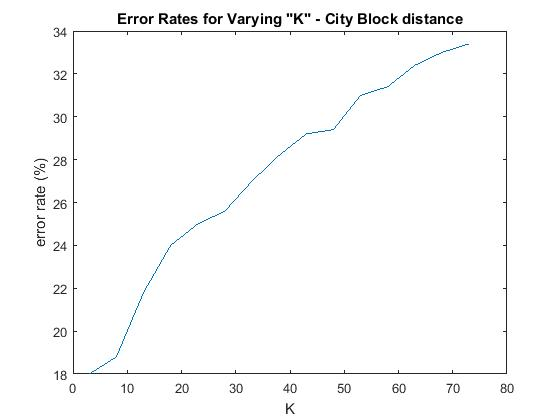
\includegraphics[width=\linewidth]{images/cb_varyingK.jpg}
    \caption{ K vs ErrorRate - City Block Distance}
    \label{fig:cb_varyingK}
    \end{figure}




\begin{table*}
\centering
  \begin{tabular}{*{15}{c}}
    \hline
    Training Data Size & Test Data Size & Error Rate\\
    \hline
    \hline
     (1)Euclidean distance \\
    \hline
   3000 & 1000 & 10.90 \\
    \hline
    6000 & 1000 & 10.10\\
    \hline
    10000 & 1000 & 9.10\\
    \hline
     7500 & 500 & 7.20 \\
     \hline
     (2) Hamming distance\\
     \hline
   3000 & 1000 & 39.30 \\
    \hline
    6000 & 1000 & 34.60\\
    \hline
    10000 & 1000 & 32.10\\
    \hline
     7500 & 500 & 33.60 \\
     \hline
     (3) City Block distance\\
     \hline
   3000 & 1000 & 12.80 \\
    \hline
    6000 & 1000 & 9.8\\
    \hline
    10000 & 1000 & 9.10\\
    \hline
     7500 & 500 & 8.20 \\

     \hline
     (4) Naive Bayes\\
     \hline
   3000 & 1000 & 23.50 \\
    \hline
    6000 & 1000 & 21.2\\
    \hline
    10000 & 1000 & 21.2\\
    \hline
     7500 & 500 & 20.2\\
    \hline\\
  \end{tabular}
 \caption{Input Sample Ratio vs Error Rates}
 \label{table:Input Sample Ratio vs Error Rates}
\end{table*}

\subsection{Observation}
From the Table 1. We understand that the error rate decreases for the increase in training sample to test sample ratio.  We also observe the euclidean distance is better than the hamming or the city block distance.

\section{Naive Bayes Classifier}

For easier understanding the images are resized to a 2D array of size samplsizex400. Each pixel is considered as an individual features for the class. We plot the histogram for the training data, with the specified bin size. Similarly when we get the test data, we compare each pixel with the histogram for that pixel for all the classes to give us a likelihood for each class. That likelihood is multiplied with the prior to get the posterior probability for that test image to be in its class. We finally choose the label which has the highest posterior probability among those calculated for that test image. The formula for posterior probability is
 
\begin{displaymath}P(C{\textsubscript k} \mid X) =   \frac{P(X\mid C{\textsubscript k}) P(C{\textsubscript k})}{ P(X)}\end{displaymath}

\begin{displaymath} posterior = \frac{ likelihood \times prior  } {evidence} \\ \end{displaymath}

 \vspace{10mm}
The likelihood is the probability that the test image is from that particular class. The prior is calculated from the training labels which are provided. The prior is the probability of the class among all the training images. Here the evidence is very marginal because the data is already normalized hence omitted. The data is only between 0 to 1.  The various error rates obtained for different training set test set data size is shown in the Table 1. The error rates for the change in bin size is shown in fig \ref{fig:ERvsBin}.


 Steps to run:
\begin{verbatim}
>> [ prediction errorRate h ] = naive( 1000, 3000 , 20 );
\end{verbatim}
Here the first argument is the test data size, second argument is the training data size and the last argument is number of bins.
 \vspace{10mm}

    \begin{figure}
    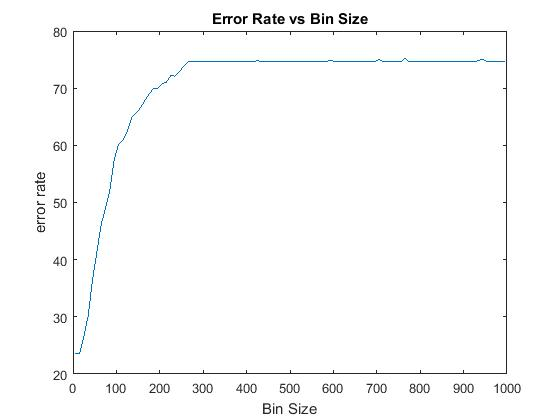
\includegraphics[width=\linewidth]{images/graph2}
    \caption{ Error Rate VS BinSize}
    \label{fig:ERvsBin}
    \end{figure}

\end{document}